% Story mode, proposed: a stage to cross ("Cross the paddies: reach the
% shrine", chapter 1). The arena is three screens wide; the camera keeps the
% player in view; opponents enter as the player passes their markers; the
% scene is won by reaching the exit. Units are the game's centimetres.
% Standalone: compiles with pdflatex.
\documentclass[tikz,border=4pt]{standalone}
\usetikzlibrary{arrows.meta,calc,decorations.pathreplacing}

\definecolor{paper}{HTML}{EFE8D8}
\definecolor{ink}{HTML}{2B2A28}
\definecolor{muted}{HTML}{6B6457}
\definecolor{ground}{HTML}{D9CDB2}
\definecolor{groundline}{HTML}{A8987A}
\definecolor{indigo}{HTML}{3E4A89}   % the player and the camera
\definecolor{ochre}{HTML}{B8862B}    % opponents

% --- The stage, in cm (the game's units); 100 cm is 1 cm on the page ----------------
\newcommand{\Half}{1800}       % arena_half: the stage runs from -1800 to 1800
\newcommand{\View}{1200}       % how much one screen shows
\newcommand{\Player}{-1500}    % where the player starts
\newcommand{\Exit}{1650}       % the shrine: reach it to win
\newcommand{\Cam}{-1200}       % the camera's centre at the moment drawn

\begin{document}
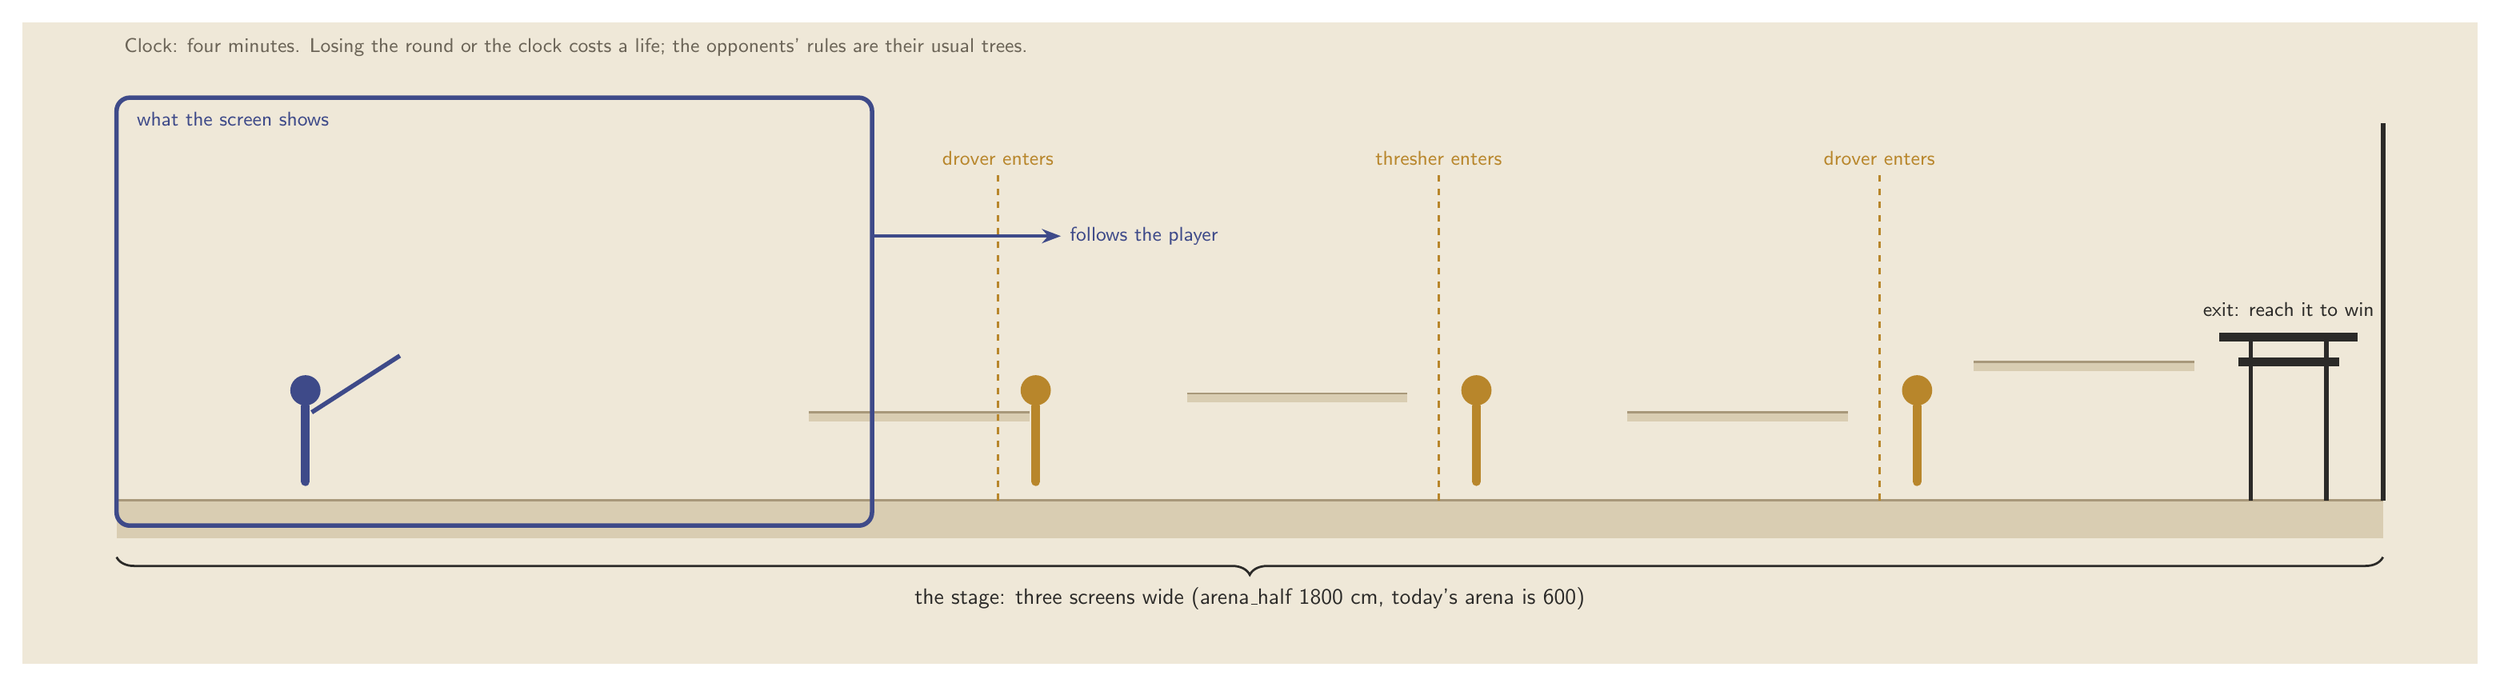
\begin{tikzpicture}[x=0.01cm, y=0.01cm, font=\sffamily, ink,
    fighter/.style={line width=4pt, line cap=round},
  ]
% --- Background ------------------------------------------------------------------------
\fill[paper] (-\Half-150,-260) rectangle (\Half+150,760);

% --- Ground and ledges (the ledges as data/maps.json writes them: x0, x1, y) -------------
\fill[ground] (-\Half,0) rectangle (\Half,-60);
\draw[groundline, line width=1pt] (-\Half,0) -- (\Half,0);
\foreach \x/\X/\y in {-700/-350/140, -100/250/170, 600/950/140, 1150/1500/220} {
  \fill[ground] (\x,\y) rectangle (\X,\y-14);
  \draw[groundline, line width=1pt] (\x,\y) -- (\X,\y);
}
% The walls at either end
\draw[ink, line width=2pt] (-\Half,0) -- (-\Half,600) (\Half,0) -- (\Half,600);

% --- Opponents' entry markers, and who enters there ---------------------------------------
\foreach \x/\who in {-400/drover, 300/thresher, 1000/drover} {
  \draw[ochre, dashed, line width=1.2pt] (\x,0) -- (\x,520);
  \node[ochre, font=\sffamily\small, above] at (\x,520) {\who\ enters};
  \draw[ochre, fighter] (\x+60,30) -- (\x+60,150);
  \fill[ochre] (\x+60,175) circle (24);
}

% --- The player -------------------------------------------------------------------------------
\draw[indigo, fighter] (\Player,30) -- (\Player,150);
\fill[indigo] (\Player,175) circle (24);
\draw[indigo, line width=2pt] (\Player+10,140) -- (\Player+150,230);

% --- The exit: the shrine ----------------------------------------------------------------------
\draw[ink, line width=2pt] (\Exit-60,0) -- (\Exit-60,260) (\Exit+60,0) -- (\Exit+60,260);
\draw[ink, line width=4pt] (\Exit-110,260) -- (\Exit+110,260) (\Exit-80,220) -- (\Exit+80,220);
\node[font=\sffamily\small, above] at (\Exit,280) {exit: reach it to win};

% --- The camera: one screen, centred on the player as far as the walls allow -----------------
\draw[indigo, line width=2pt, rounded corners=6] (\Cam-\View/2,-40) rectangle (\Cam+\View/2,640);
\node[indigo, font=\sffamily\small, anchor=north west] at (\Cam-\View/2+20,630) {what the screen shows};
\draw[indigo, -{Stealth[length=3mm]}, line width=1.4pt] (\Cam+\View/2,420) -- ++(300,0) node[right, font=\sffamily\small] {follows the player};

% --- Annotations (last) --------------------------------------------------------------------------
\draw[decorate, decoration={brace, amplitude=8pt, mirror}, line width=1pt]
  (-\Half,-90) -- (\Half,-90) node[midway, below=10pt] {the stage: three screens wide (arena\_half \Half\ cm, today's arena is 600)};
\node[font=\sffamily\small, text=muted, anchor=west] at (-\Half,720)
  {Clock: four minutes. Losing the round or the clock costs a life; the opponents' rules are their usual trees.};
\end{tikzpicture}
\end{document}
